% !TEX TS-program = xelatex
% !TEX encoding = UTF-8 Unicode
% ================================================
%  上海交通大学 研究生工作周报
%  编译: xelatex → bibtex → xelatex → xelatex
% ================================================

\documentclass{sjtuweekly}
\usepackage{booktabs}
\usepackage{tabularx}
\usepackage{array}
\usepackage{enumitem}
\usepackage{float}

\renewcommand{\thefigure}{\arabic{figure}}
\renewcommand{\thetable}{\arabic{table}}

\bibfile{bib/database}

\member{霍锦龙}
\weeknum{xx}

\begin{document}

\makeweeklytitle

% ================================================
\section{一、本周工作概要}

\subsection*{1.1\quad 论文复现： HCF 建模}

基于``Selective Deployment of Bidirectional Hollow-Core Fibers in Hybrid SMF/HCF Optical Networks'' 文献建模. 复现并完成新情景下的建模和metrics讨论优化:


\textbf{研究问题：} 
与传统的统一部署相比，BiDi-HCF的选择性部署如何影响全网吞吐量、每Tbps功耗和收发器分配讨论.

针对当前单一模态fabric(SMF)的不足,空心光纤(HCF)如何通过更低的衰减(瑞利散射)和非线性特征极大提升光路的GSNR,可以让部署利用消耗更低的Transponder,如ZR+替代LongHaul. 显而易见,不需要替换所有SMF,因此,文章的思路是将关键链路替代(metric为最小化归一后的transponder功率和频谱时隙占用):

\begin{equation}
  J = \alpha \cdot \frac{P_{e,i}}{P_{e,\max}} + \beta \cdot \frac{S_i}{S_{\max}}
  \label{objective_function}
\end{equation}

\textbf{场景建模：} 
单一模态SMF(uni-SMF);单一空心光纤(uni-HCF);单一双向HCF(Bidi-HCF);混合单一模态fabric和单一空心光纤;混合单一模态和双向HCF.

SMF模型设置参考: ``Semrau et al., 2019, A closed-form approximation of the Gaussian noise model in the presence of inter-channel stimulated Raman scattering"

HCF模型设置参考: ``Poggiolini & Poletti, 2022, Opportunities and challenges for long-distance transmission in hollow-core fibres"

BiDi-HCF模型参考: ``P. Torres-Ferrera et al., Single-fiber bidirectional transmission using 400g coherent digital subcarrier transceivers''

验证模型参考:`` X. Zhang et al., 273.6 tbit/s real-time s+c+l-band samewavelength bidirectional wavelength division multiplexing transmission in anti-resonant hollow-core fiber"

Transponder模型设参考:``Infinera Corporation, Infinera cloudwave chm2t/chm1t multiservice transponder – data sheet, Data sheet (PDF), Accessed 2026-04-19.''

RMSA优化模型:每一个场景都运行了50次, 同时针对routing(k-shortest-path heuristic), modulation, spectrum assignment(First-Fit)进行建模.

仿真建模:拓扑EU19, 流量速率[400, 800, 1200, 1600] Gbps 对应概率[0.25, 0.4, 0.25, 0.1]

性能指标: Power consumption per Tbps, Total served traffic, Percentage of transponder allocation 

\textbf{关键发现和结论：} 

优先功率时ZR+是更好地选择,优先频谱时LH更好; HCF全面优于SMF; 10-50\%链接升级为Bidi-HCF会降低5-20\%系统功率消耗; 50\%的Bidi-HCF 较SMF提升40\%; 50\%的Bidi-HCF 可以达到80\%全HCF的设置; 每Tb级别流量系统功耗降低约20\%.


\subsection*{1.2\quad 实验复现}

% \begin{enumerate}
%   \item \textbf{路由可学习且方向稳定:} 同一输入，训练前后 71.1\% 路由决策一致性分析:层 0: 93.4\% 到 层 39: 54.5\% 图\ref{fig:routing}A 所示.
%   \item \textbf{路由集中化:} 从预训练前到微调后的活跃专家数大幅下降, 从1到层38: 专家激活从161到68(可以作为ocs降低资源收集和计算复杂度的部分依据)图\ref{fig:routing}B 所示.专家256/均被某层使用.专家 41 激活次数最多有 32 次分配.
%   \item \textbf{协同激活:} Top-20 共激活对训练后全部持续存在，41, 151, 224号专家始终作为适配的激活专家.

% \end{enumerate}

\begin{figure}[htbp]
  \centering
  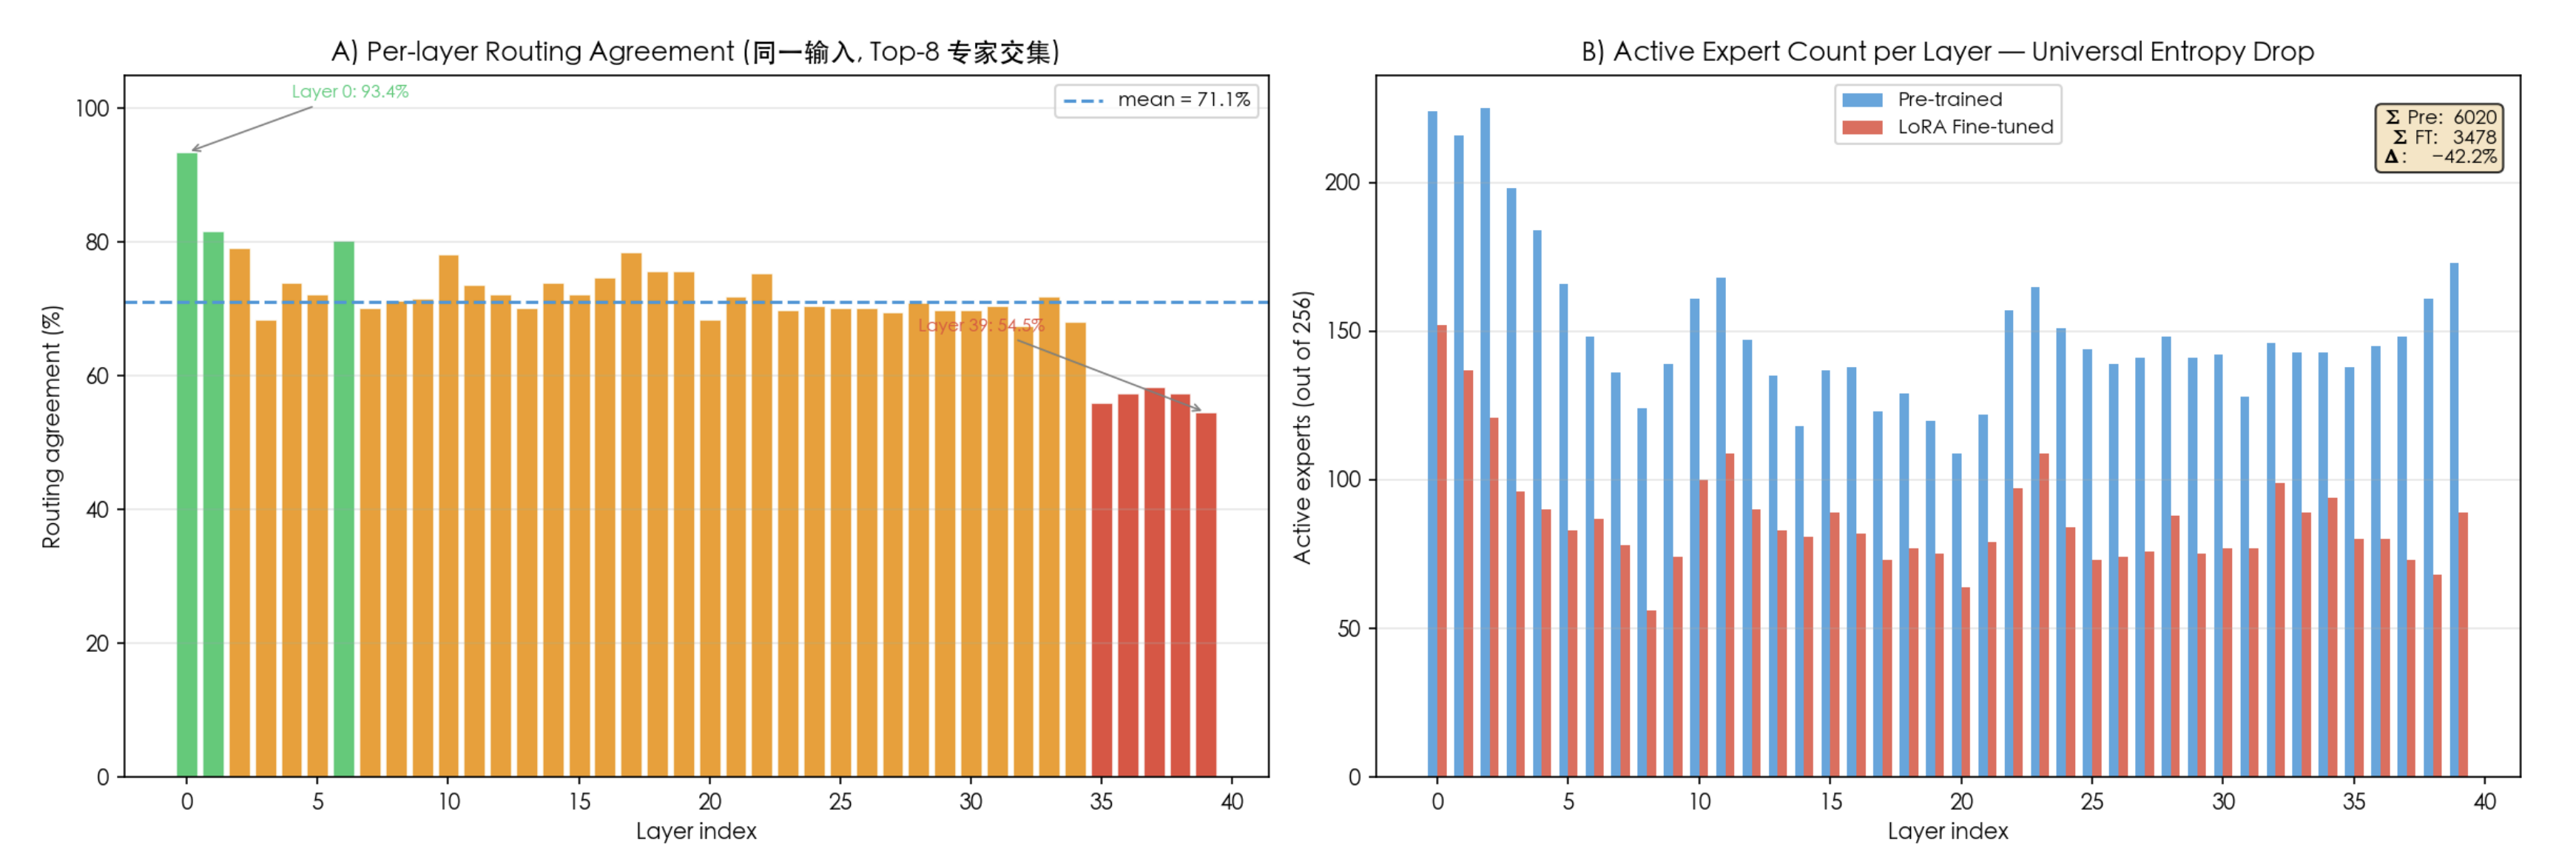
\includegraphics[width=\linewidth]{figures/fig1.png}
  \caption{训练前后路由分布对比}
  \label{fig:routing}
\end{figure}

% ================================================
\section{二、遇到的问题与讨论}

\subsection*{2.1\quad 统计角度}

\begin{enumerate}[label=(\arabic*), leftmargin=*]
  \item \textbf{构造数据较少:} 当前的 71\% 训练前后一致基于比较脆弱的假设,即当前的数据样本比较少.同时考虑到有相关文献指出应用于 OCS 需要算法或验证模型具备一定预测性/泛化性.即 gate 计算前预测未见 token 的专家集.从这个角度出发, 严格来说,两者数学上不同，前者无法推导后者.但是,在当前的预训练/后训练下,刨除多模态moe的影响,单一模态具备类似数学上的预测性.也就是具备一定程度上的可推广性.

  \item \textbf{训练退化:} 训练时有时会 checkpoint 崩溃，这里还没有涉及退化崩溃前后专家下降的贡献度讨论.
  \item \textbf{训练一致性:} 当前是基于模型进行后训练(post),而非从一个开始就进行训练.从头开始训练的LLM token分布还要再进行细致的讨论.
\end{enumerate}

\subsection*{2.2\quad 建模角度}

\begin{enumerate}[label=(\arabic*), leftmargin=*]
  \item \textbf{硬件粒度错配:} 考虑到活跃专家总数下降但是并不会减少单 token 电路需求.例如 Top-8 每 token 始终需 8 专家. 那么后续可能还要考虑在OCS场景下的并发token在同一时间窗内的专家集重叠度和资源收集以及调度问题.
  \item \textbf{缺乏OCS延迟预算:} 很多文献都指出MEMS OCS 切换 在ms级别，但是单层推理在微秒级, $\tau_{\text{reconf}} \gg \tau_{\text{compute}}$ .所以单 token 粒度预触发物理是否可行, 需明确硬件假设就是上次的讨论内容，或粗化到批次粒度（MixNet 思路）.
  \item \textbf{MoE流量矩阵和OCS重配置适配度:} 分布式 MoE 是 All-to-All 集合通信. 部分文章中指出 OCS 在一定程度上要支持批次内的置换矩阵(分解流量矩阵)，而非单个专家对之间的连线(性价比不高).后续可能要考虑 A2A 流量矩阵的稀疏度来决定批次内训练/推理的拓扑设置.

\end{enumerate}

% ================================================
\section{三、工作计划}

\begin{table}[H]
\centering
\small
\begin{tabularx}{\linewidth}{@{}>{\raggedright\arraybackslash}p{0.62\linewidth}>{\centering\arraybackslash}X@{}}
\toprule
\textbf{内容} & \textbf{预期产出} \\
\midrule
\textbf{多样化微调:} 使用跨领域样本再次微调，确保生成数据分布和路由偏好不退化，复测活跃专家/熵是否仍下降 & checkpoint 失效前后的分布讨论 \\
\textbf{硬件建模:} 选定 $\tau_{\text{reconf}}$（MEMS/photonic/SOA）和 $\tau_{\text{compute}}$（目标 batch），计算期望延迟公式，判定物理可行性 & 项目是否有物理意义 \\
\textbf{构建预测器:} 用前一层的 expert set 或 pre-gate activations 做线性 probe 预测当前层 expert set，对比 chance baseline（3.1\%）和 SOTA（93--97\%） & 验证MoE专家网络token可预测性的上下界 \\
\textbf{系统对标:} 切换分析单元到并发 token 专家集重叠度；与 MixNet / pre-attention predictor 并列对比；多租户混合流量压力测试 & 在系统社区中的定位 \\
\bottomrule
\end{tabularx}

\caption{后续计划}
\label{tab:plan}
\end{table}


\printbib

\end{document}
